%%%%%%%%%%%%%%%%%%%%%%%%%%%%%%%%%%%%%%%%%%%%%%%%%%%%%%%%%%%%%%%%%%%%%%%%%%
%%%%%                         CHAPITRE 6                            %%%%%%
%%%%%%%%%%%%%%%%%%%%%%%%%%%%%%%%%%%%%%%%%%%%%%%%%%%%%%%%%%%%%%%%%%%%%%%%%%

\lhead[\fancyplain{}{\leftmark}]%Pour les pages paires \bfseries
      {\fancyplain{}{}} %Pour les pages impaires
\chead[\fancyplain{}{}]%
      {\fancyplain{}{}}
\rhead[\fancyplain{}{}]%Pour les pages paires 
      {\fancyplain{}{\rightmark}}%Pour les pages impaires \bfseries
\lfoot[\fancyplain{}{}]%
      {\fancyplain{}{}}
\cfoot[\fancyplain{}{\thepage}]%\bfseries
      {\fancyplain{}{\thepage}} %\bfseries
\rfoot[\fancyplain{}{}]%
     {\fancyplain{}{\scriptsize}}


%%%%%%%%%%%%%%%%%%%%%%%%%%%%%%%%%%%%%%%%%%%%%%%%%%%%%%%%%%%%%%%%%%%%%%%%%%
%%%%%                      Start part here                          %%%%%%
%%%%%%%%%%%%%%%%%%%%%%%%%%%%%%%%%%%%%%%%%%%%%%%%%%%%%%%%%%%%%%%%%%%%%%%%%%

\chapter{Application to boxing, using action cameras}
\label{ch:6}

%==============================================================================	Résumé du chapitre

\begin{center}
\rule{0.7\linewidth}{.5pt}
\begin{minipage}{0.7\linewidth}
\smallskip

\textit{Boxing is a challenging sport for motion analysis, because movements are fast, 3 dimensional, and involves the whole body. Moreover, it is usually not possible to equip a boxer with markers, lightning conditions and large capture volumes make the classic marker-based difficult, research-grade cameras are too cumbersome to set up in a timely way and lower-end cameras can't be synchronized by hardware, nor with a flash in the context of a competition.\newline\newline
The objective of the study was to verify whether it is possible to accurately measure Key Performance Indicators (KPIs) in boxing, with a markerless protocol and under suboptimal conditions. This was concurrently validated with a marker-based protocol. A secondary goal was to compare the impact on result quality of a markerless analysis with post-calibration and post-synchronization, to the impact of choosing a different 2D pose estimation model. We conclude that KPIs are remarkably well evaluated in all conditions, although the choice of the 2D pose estimator is more influential than the protocol. \newline \newline
This chapter is adapted from the poster presented at the congress of the European College of Sport Science (ECSS): "A 3D markerless protocol with action cameras – Key performance indicators in boxing" \cite{Pagnon2022c}.
}

%\smallskip
\end{minipage}
\smallskip
\rule{0.7\linewidth}{.5pt}
\end{center}

\clearpage

\minitoc

\vspace*{3cm}

\begin{figure}[hbtp]
	\centering
	\def\svgwidth{1\columnwidth}
	\fontsize{10pt}{10pt}\selectfont
	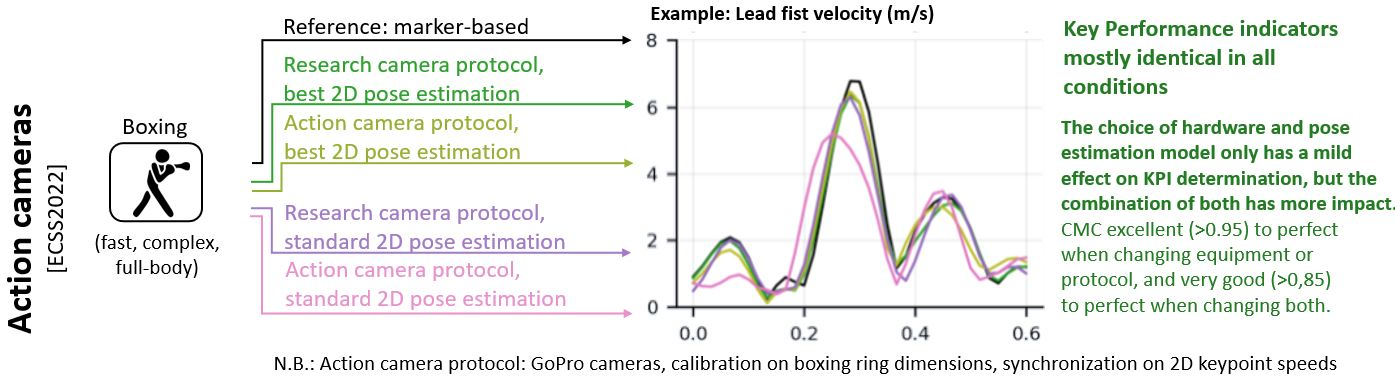
\includegraphics[width=\linewidth]{"../Intro/Figures/Fig_VisAbstract4.JPG"}
      \caption{Visual abstract for the assessment of KPIs in boxing with Pose2Sim \cite{Pagnon2022c}.}
	\label{fig_visabstract4}
\end{figure}

\newpage






\section{Objectives}

\subsection{Key Performance Indicators in boxing}

Key Performance Indicators (KPIs) are a set of variables which need to be measured in priority, in order to assess performance, or to evaluate main areas where work is needed. Although they are more known in the fields of management or of the industry, identifying them is also important in sports \cite{Hughes2002,Butterworth2013}. Determining them would typically be done in two steps. First, through discussions with coaches, who usually have a subjective, but nevertheless very fine and comprehensive understanding of their sport. Then, the most relevant of these variables can be selected, for example by Principal Component Analysis (PCA) \cite{Hotelling1933}. PCA allows for grouping the variables that explain most of the performance, and excluding the others \cite{ODonoghue2008}.

However, this approach has the disadvantage that prior to pursuing any further statistical analysis, all the potential variables first need to be extensively recorded. Only then, the most relevant ones can be determined. Moreover, it might lead to the selection of indicators which can be hard to retrieve, or be not intuitively meaningful as they potentially consist in the linear combination of some seemingly unrelated variables. In this case, one can choose the performance indicator most associated with each principal component \cite{ODonoghue2008}. Other methods exist, such as exclusive expert coach opinion, hierarchical models based on breaking down individual techniques, or notational analysis based on scoring events and actions along a competition, or other inferential statistics such as regression analysis, and more \cite{Hughes2002,Butterworth2013}.

KPIs in boxing can be separated into several categories: action annotations (such as points scored, number of recorder jabs punches or dodging by leaning backwards \cite{Thomson2013}), anthropometric KPIs (such as long arm length and high muscle percentage \cite{Chaabene2015}), physiological (such as high velocity at maximal oxygen uptake and high anaerobic power \cite{Chaabene2015}), or biomechanical (such as ground reaction force of the rear leg before execution of a cross punch, activation of the latissiums dorsi during the hook punch, or extension of the elbow at the end of the execution of the jab \cite{Lenetsky2020}). 

Among all these KPIs, we focus on a subset of the biomechanic ones, namely kinematics. Ultimately, a decisive aspect in a punch is its speed, which determines how powerful it is (along with force), and how difficult it will be for the opponent to dodge it. However, speed is not generated the same way in jabs as in hooks, since one is a mostly translational movement whereas the other is mostly rotational. \cite{Lenetsky2020} broke down the phases of both techniques. Among other body motions, the jab involves translating the lead foot toward the target, then the pelvis and the torso follow, while the lead arm flexes at the elbow to store elastic energy prior to throwing the punch. Finally, the elbow extends, until the fist is brought into contact with the target. Regarding the rear hook, it starts with flexion of the rear knee, while the pelvis and torso rotate horizontally away from the target. Then the motion is reversed, as the knee extends and the pelvis and torso rotate toward the target. Lastly, the attacking arm abducts at the shoulder until the fist reaches the target. 

As a consequence, it seems like the lead foot translation, the pelvis translation, the lead elbow extension, and the lead fist velocity would consist in good KPIs for the jab, and the rear knee flexion, the pelvis rotation, the rear shoulder extension, and the rear fist velocity would be valuable to estimate for the rear hook.


\subsection{Limits of research-grade systems in competitions}

When fine kinematic analysis is needed, the de facto method is marker-based motion capture. However, it is not appropriate in sports, as it involves laying markers directly on the skin, which is not conceivable during a match or a sparring session. It is intrusive and cumbersome, and usually involves specific environment conditions. Moreover, markers can fall off the body when the athlete is sweating or moving fast. As a consequence, it is important to investigate markerless techniques. 

Another constraint of sports analysis is the capture system, which needs to be discrete and installed swiftly. As a consequence, research grade video systems such as Qualisys are not appropriate: they involve setting up large cameras and stands, with cumbersome power and synchronization cables, and they need at least two trained operators to set them up and to adjust their parameters. They are also very expensive, while their framerate and resolution are not very good. On the other end, consumer-grade action cameras such as GoPros are very small, don't require any cabling, and the operator has nothing to do but clicking the recording button. They are also cheap, and offer remarkably high framerate, resolution, and image quality. However, their battery does not last more than an hour, they don't come with calibration, and until recently, no synchronization solution existed. There is also no centralized visual feedback on the recording.





•Classic marker-based calibration is impossible? (cameras at a distance or outdoors)

•Usual synchronization methods are not feasible? (no cables, no flash, no clap)

Subsidiary question: Does the choice of the 2D pose estimation model matter?



Markers, Cameras et setup, Calibration, synchronization, Feedback


étude avec imus \cite{Haralabidis2020}


In boxing, the analysis of the kinematics of the upper body is of particular interest, because it is the main source of power in punches. The main objective of this study was to evaluate the accuracy of the 3D kinematic analysis of the upper body in boxing, using a markerless protocol and action cameras. The secondary objective was to compare the impact on result quality of a markerless analysis with post-calibration and post-synchronization, to the impact of choosing a different 2D pose estimation model.



shadow boxing


% Calibration remains a challenging task in daylight, at a distance, with non research-grade cameras, and in a sports scene. It could be useful to make it more robust, either by implementing the Aniposelib library \cite{Karashchuk2020}, or by calibrating automatically on people’s limb length \cite{Liu2022a}.

% La calibration sera impossible si vous êtes trop loin. Les marqueurs réfléchissants ne réfléchiront pas la lumière des caméras (à tester : marqueurs actifs).  
% Si vous voulez effectuer une post-calibration avec un checkerboard (avec cette méthode par exemple), il faudra que le checkerboard soit assez grand pour qu’il soit bien détecté. Une règle simple : pour avoir de bons résultats, la largeur du checkerboard doit remplir au moins un cinquième de l’image. Si vous voulez couvrir une scène de 20 m, il faudra un checkerboard de 4 m de large...  
% Autre solution non testée : Calculer hors manip les paramètres intrinsèques des caméras vidéo. En manip, placer côte à côte des caméras MoCap Arqus et vidéo Miqus, faire la calibration des Arqus (plus performantes), et ajouter une translation dans les paramètres extrinsèques des Arqus pour avoir ceux des Miqus. 


% Adding muscles which were stripped from the skeleton in the OpenSim model could allow for joint kinetics prediction. Neural networks could be trained to estimate ground reaction forces from kinetics on specific tasks, without the use of a force platform [Oh2013, Johnson2018, Mundt2019].
% Using Xsens markers hidden by clothes in Kinovis? Although not gold-standard


\subsection{Objectives}

\cite{Haralabidis2020} monitored the effect of fatigue on punching performance by fusing the outputs of IMUs with those of OpenPose processed videos. However, is this is not a full markerless protocol, we opt for performing kinematic analysis with Pose2Sim \cite{Pagnon2022b} (see \autoref{ch:3}).

Concurrently validating the accuracy of KPI measurements in boxing with suboptimal markerless protocols.


\section{Methods}
\subsection{4 conditions}
\blindtext

\subsection{Pose-calibration on ring dimensions}
\blindtext

\subsection{Post-synchronization on 2D movement speeds}
\blindtext

\subsection{GoPro spatio-temporal base into Qualysis'}
\blindtext

\subsection{Statistical analysis}
\blindtext


\section{Results}
\blindtext


\section{Discussion}
\subsection{Equipment and protocol vs. pose estimation model}
\blindtext

\subsection{Pros and cons of different systems}

Auto-calibration with person?

Cloud computing?

Temporal consistency?

Shape information for less cameras?

Rolling shutter: Pour les GoPros, la fréquence de roll du shutter de haut en bas est approxivement la même que la fréquence d'acquisition, donc vu qu'on peut filmer jusqu'à 240 Hz en full HD, 120Hz en 4K, et 60Hz à 5.3k, je doute que ce soit un vrai problème...
Pas de retour visuel instantanné
Synchro : nouvelles avec GPS, sinon méthodes
Calib : Mieux qu'avec Qualisys en plein air

\blindtext
